%% LyX 2.2.3 created this file.  For more info, see http://www.lyx.org/.
%% Do not edit unless you really know what you are doing.
\documentclass[english]{article}
\usepackage[T1]{fontenc}
\usepackage[latin9]{luainputenc}
\usepackage{geometry}
\geometry{verbose,tmargin=2cm,bmargin=2cm,lmargin=2cm,rmargin=2cm,headheight=2cm,headsep=2cm}
\setlength{\parindent}{0bp}
\usepackage{amssymb}
\usepackage{graphicx}
\usepackage{babel}
\begin{document}

\section{Filtro pasabajos}

Se pidi� aplicar a un filtro RC de frecuencia de corte $f_{0}=64\,(kHz)$
una onda cuadrada de $10\,V_{pp}$ con frecuencia de $f=32\,(kHz)$
. Los resultados obtenidos empiricamente fueron los que se muestran
en la figura \ref{2_1}. A su vez, se calculo la transferecia del
circuito idealmente resultando ser:

\begin{equation}
H(s)=\frac{1}{1+sRC}\label{eq:2_4}
\end{equation}

Si simulamos la transferencia del circuito en LTSpice, el resultado
es el que se ve en la figura \ref{2_4}.

\begin{figure}[h]
\caption{Resultados}
\label{2_1}

\end{figure}

\begin{figure}[h]
\begin{centering}
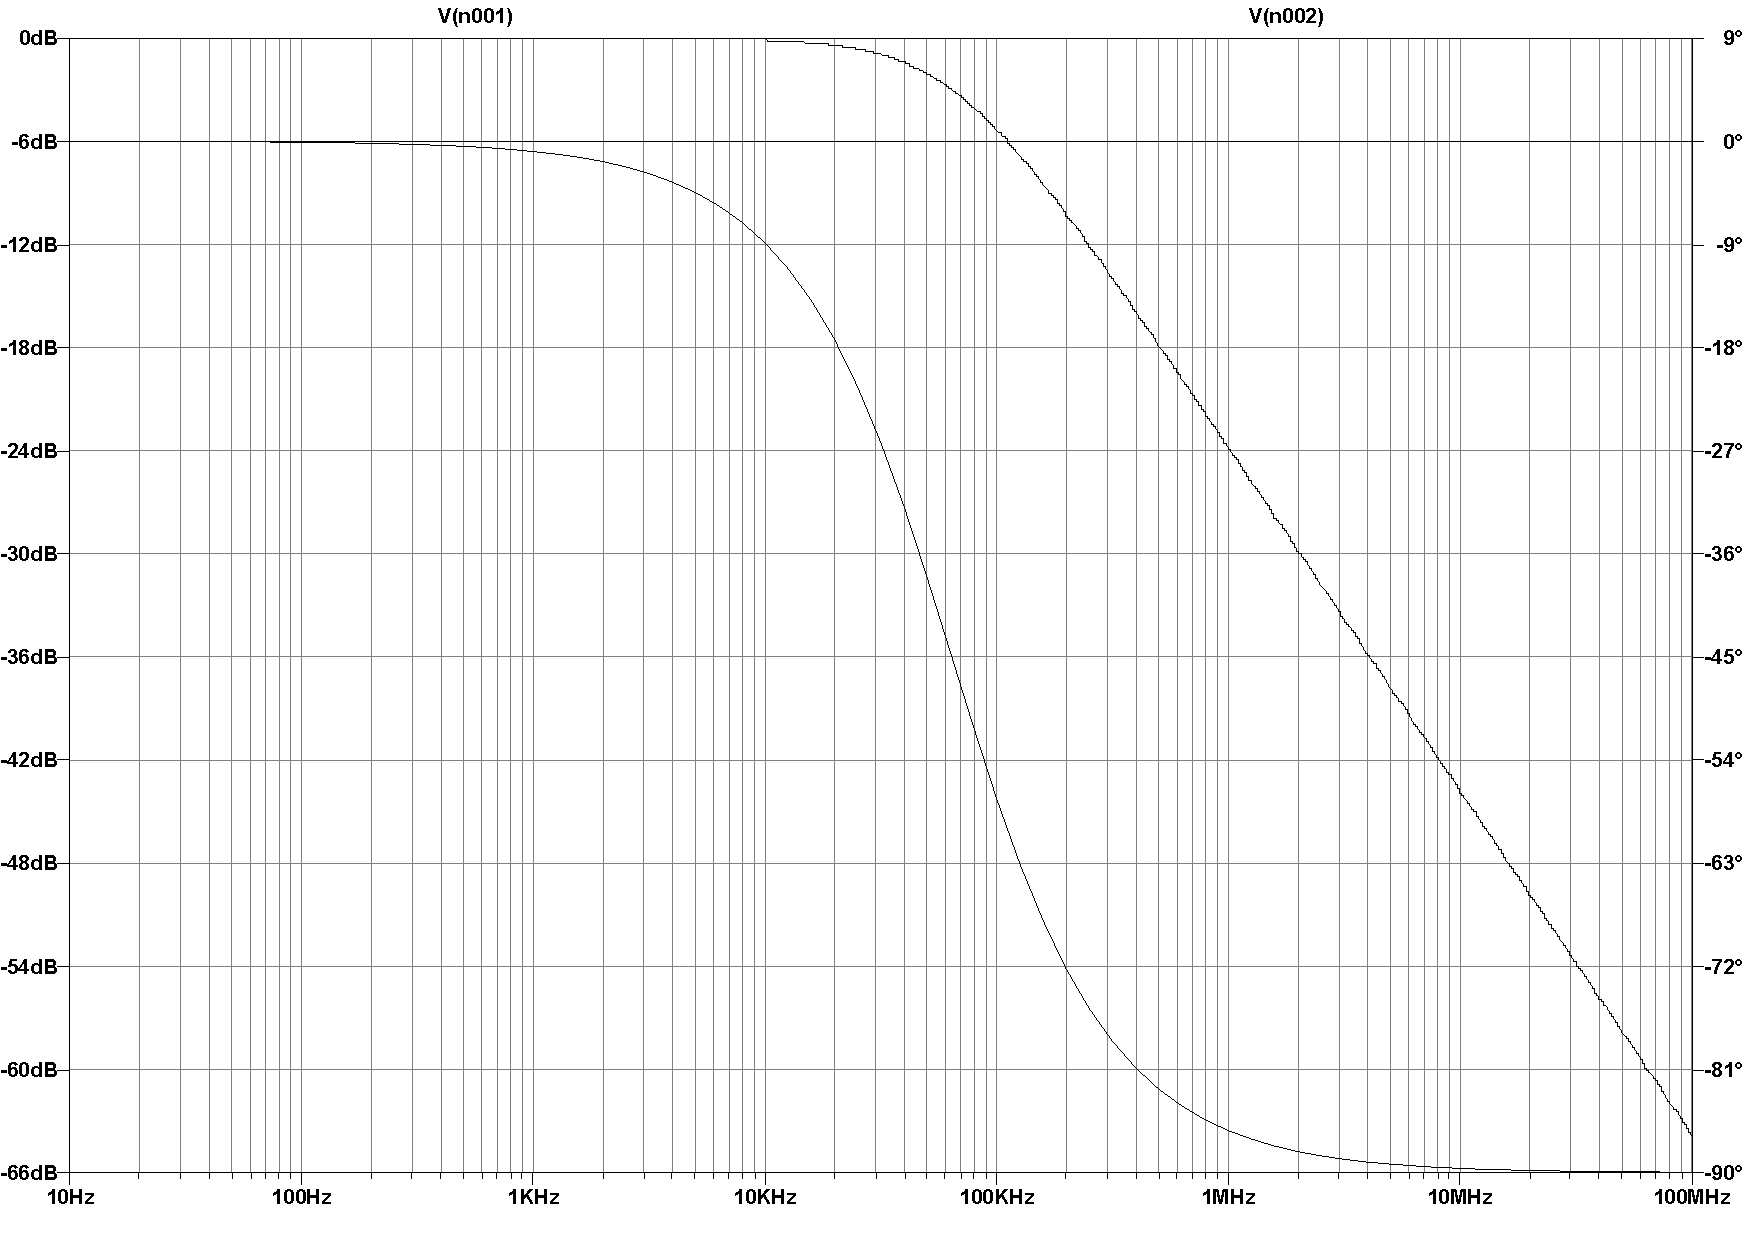
\includegraphics[scale=0.4]{plot}
\par\end{centering}
\caption{Simulacion LTSpice}
\label{2_4}

\end{figure}

\subsection{Calculo de arm�nicos}

Si queremos ver como reacciona el circuito a una se�al cuadrada, debemos
calcular primero como afecta nuestro circuito a la onda de entrada.
Como sabemos que la onda es una cuadrada, haciendo su descomposici�n
de suma de se�ales trigonometricas, los coeficientes de Fourier resultan
ser:

\[
a_{0}=0
\]

\[
a_{n}=0
\]

\[
b_{2n-1}=\frac{20}{(2n-1)\pi}
\]

\[
b_{2n}=0
\]

Por lo tanto, la onda cuadrada se puede expresar en el espacio temporal
como se ve en la expresi�n \ref{eq:2_1}. Sin embargo, podemos ver,
por temas de idealizacion, que una se�al cuadrada ideal, se puede
aproximar por una suma de t�rminos finitos de senoidales, por lo tanto,
si aproximamos la cuadrada con 10 terminos, podemos ver como la aproximacion
van quedando mas parecidas, esto se muestra en la figura \ref{2_2}.
A medida que agreguemos mas t�rminos a nuestra suma, menos sera la
diferencia con una onda cuadrada ideal. No obstante, hay que tener
en cuenta que, como fue visto en Matem�tica V, al tener una discontinuidad
no evitable cada $\frac{T}{2}$, siendo \emph{T} el per�odo de la
se�al, se generaran sobrepicos en los puntos de discontinuidad. por
ende, si llamamos \emph{x(t)} a la funci�n cuadrada ideal e \emph{y(t)}
a su aproximaci�n por senoides, \emph{x(t)} ser� igual a \emph{y(t)
}en todos los numeros reales exceptuando los puntos de discontinuidad.
Esto quiere decir, que es posible que al trabajar con ondas cuadradas,
se encuentren sobrepicos.

\begin{equation}
x(t)\sim\sum_{n=1}^{\infty}\frac{20}{(2n-1)\pi}sin\left(2\pi(2n-1)f_{0}t\right)\label{eq:2_1}
\end{equation}

\begin{figure}[h]
\begin{centering}
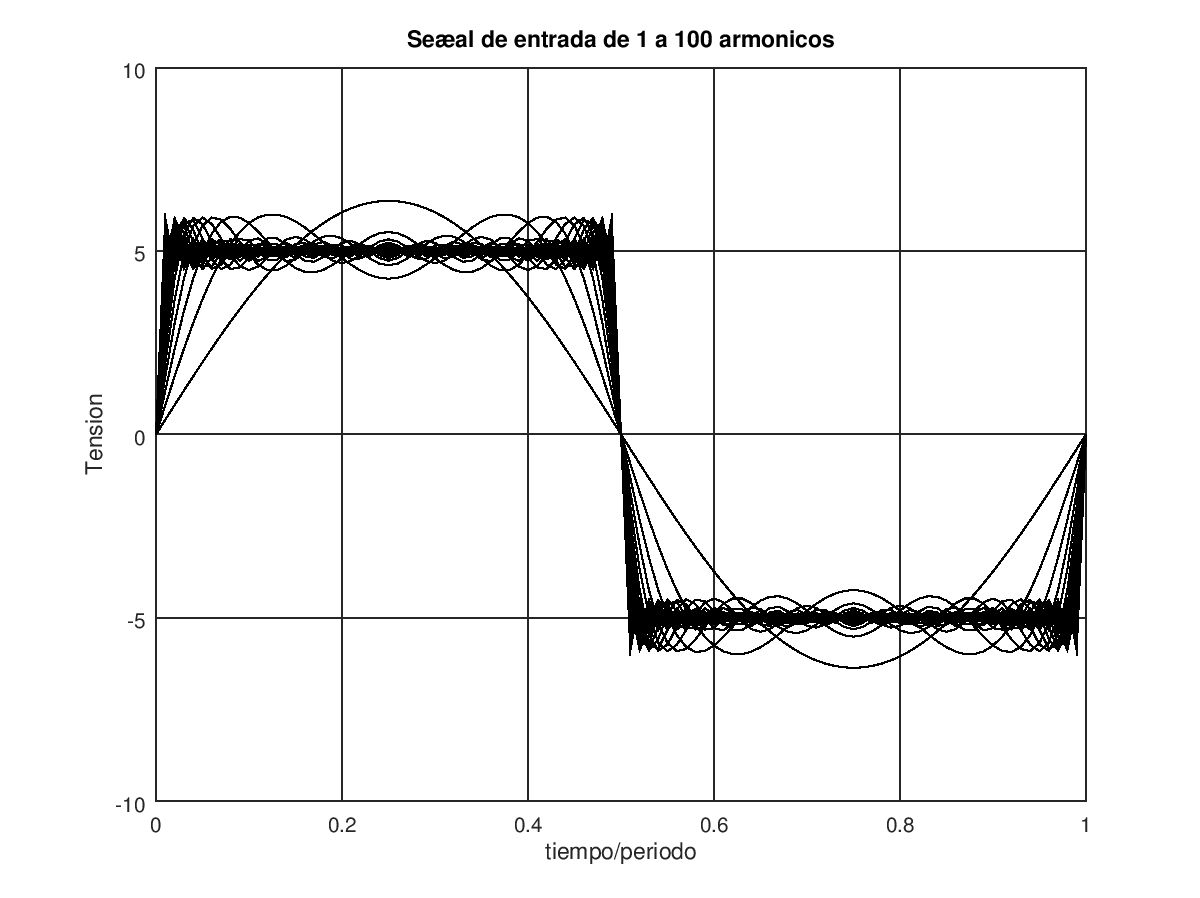
\includegraphics[scale=0.5]{Square}
\par\end{centering}
\caption{Representaci�n de onda cuadrada mediante suma de senoidales}
\label{2_2}
\end{figure}

Debido a que la entrada es una funci�n continua a trozos de per�odo
\emph{T, }entonces:

\[
y(t)\sim\sum_{n=1}^{\infty}\left|b_{2n-1}\right|\left|H\left((2n-1)f_{0}\right)\right|cos\left[2\pi(2n-1)f_{0}t+\phi((2n-1)f_{0})+\theta_{2n-1}\right]
\]

\begin{equation}
b_{2n-1}=\left|b_{2n-1}\right|e^{i\theta_{2n-1}}\label{eq:3}
\end{equation}

\[
H(f)=\left|H(f)\right|e^{i\phi(f)}
\]

A su vez;

\begin{equation}
H(f)=\frac{1}{1+i2\pi fRC}\label{eq:2}
\end{equation}

Por lo tanto, haciendo calculos de las ecuaciones \ref{eq:3} y \ref{eq:2},
concluimos que:

\[
\phi(f)=-arctg(2\pi fRC)
\]

\[
H(f)=\frac{1}{\sqrt{(2\pi fRC)^{2}+1}}
\]

\[
\theta_{n}=0
\]

Finalmente, podemos escribir la salida como la ecuacion \ref{eq:2_3}
y graficamente se ve como la figura \ref{2_3}.

\begin{equation}
y(t)\sim\sum_{n=1}^{\infty}\frac{20}{(2n-1)\pi\sqrt{\left(2\pi(2n-1)f_{0}RC\right)^{2}+1}}cos\left(2\pi(2n-1)f_{0}t-arctg\left(2\pi(2n-1)f_{0}RC\right)+\frac{\pi}{2}\right)\label{eq:2_3}
\end{equation}

Teniendo en cuenta que $f_{0}=\frac{1}{2\pi RC}$ entonces;

\[
y(t)\sim\sum_{n=1}^{\infty}\frac{20}{(2n-1)\pi\sqrt{\left(2n-1\right)^{2}+1}}cos\left(2\pi(2n-1)f_{0}t-arctg\left(2n-1\right)+\frac{\pi}{2}\right)
\]

\begin{figure}[h]
\begin{centering}
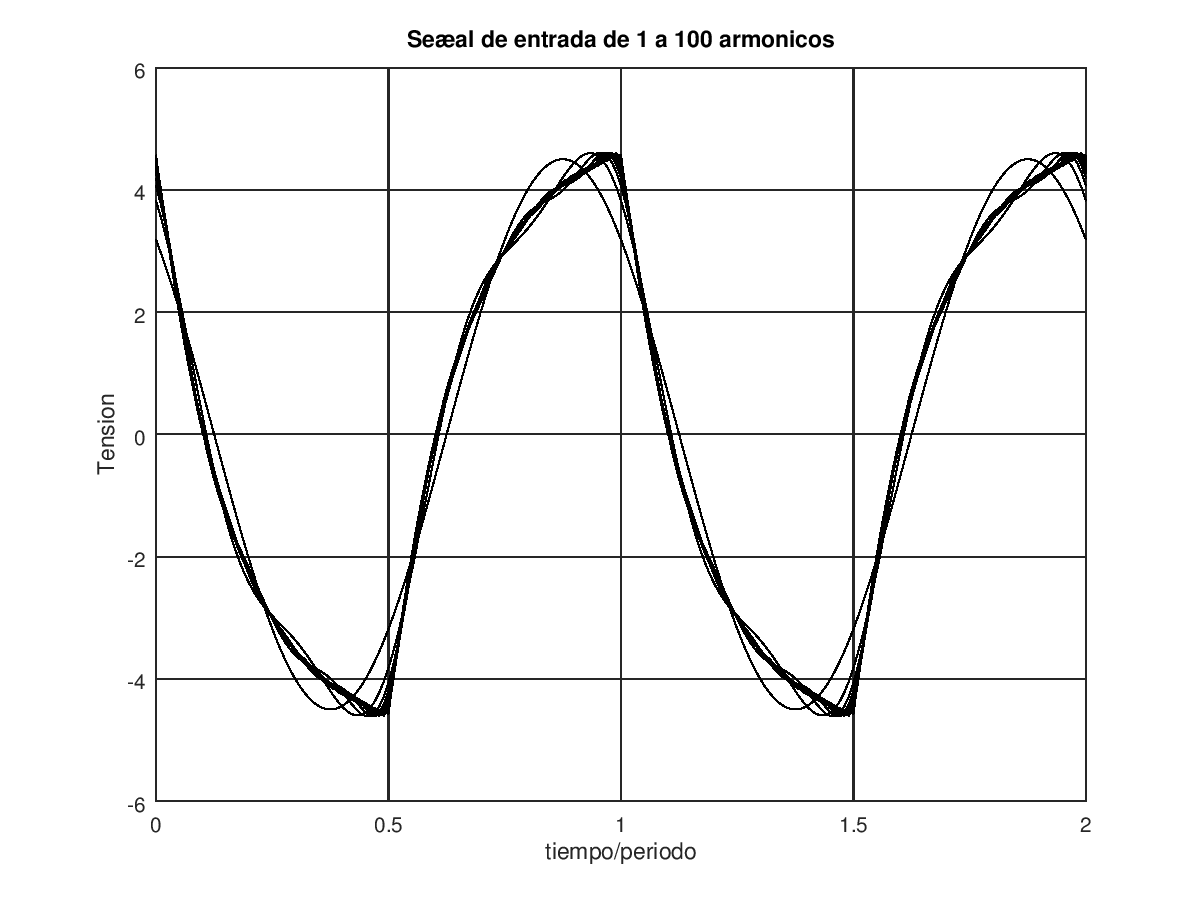
\includegraphics[scale=0.5]{out_calc}
\par\end{centering}
\caption{Salida del RC en arm�nicos}
\label{2_3}
\end{figure}

\subsection{Circuito como Integrador}

Como ya sabemos, un circuito integrador es aquel que cumple que su
funcion transferencia sea $H(s)=\frac{1}{s}$, como vemos en la ecuacion
\ref{eq:2_4}, nuestro circuito no posee esa transferencia, sin embargo,
si procuramos movernos en un intervalo donde \emph{sRC }sea lo suficientemente
grande comparado con 1, podremos aproximar a una funcion transferecia
integradora. Es decir;

\[
Si\,\,sRC\ggg1\Longrightarrow H(s)=\frac{1}{1+sRC}\approx\frac{1}{RC}\frac{1}{s}
\]

Por ende, si cambiamos al espacio de frecuencias, procurando que $2\pi fRC\ggg1$
podemos obtener la transferencia de un circuito integrador. En particular,
para $R=2.5(k\Omega)\,y\,C=1(nF)$ debemos concluir que para una frecuiencia
$f_{a}\ggg63(kHz)$, nuestro circuito se comportar� como un integrador.


\end{document}
